% !TEX root = ../../thesis.tex

\cleartoleftpage
\includepdf{../media/chapter_illustration/poppy_prairie_2.pdf}

\chapter{Open diffusion of Poppy: perspectives and challenges} % (fold)
\label{cha:diffusion}

\section{Introduction} % (fold)

Poppy was initially designed with a scientific objective, aiming to be a new experimental platform opening the possibility to systematically study the role of morphology in sensorimotor control, in human-robot interaction and in cognitive development. Yet, until recently it was complicated because building a robot relied on heavy and costly manufacturing techniques. 3D printing has changed the landscape of what is possible: the design of Poppy transposed it to humanoid robotics and we developed complementary open source electronic and software. As we saw in chapter~\ref{cha:changing_morphology}, it allows to explore new body shapes in just a few days.
In addition, it enables and simplifies the experimentation, the reproduction and the modification of the morphology in research laboratories. It also allows collaborative working, sharing and replication of the results between laboratories.

On the scientific aspect, the ambition is to become a reference platform for benchmarking and dissemination of scientific results. Also, the simple design of Poppy also targets non-engineering scientists so humanities, biologist and so on can contribute to the robotics field by using Poppy as experimental tool.
Moreover, thanks to the fact that it integrates advanced and yet easily accessible techniques in an embodiment that motivates students and the wider public, this platform also meets a growing societal need: education and training in technologies combining computer science, electronics and mechanics, as well as a training tool to the emergent revolutionary 3D printing process. With its openness, its design and its rather low-cost, Poppy provides a unique context for experimentation and learning of these technologies in a Do-It-Yourself (DIY) approach.
Finally, the possibility to easily modify both the hardware and the software also makes Poppy a useful tool for artistic projects working with interactive computerized installations.

% Poppy is an open source/open science project, even if the technology developed have a high potential to be relevant in Art, Education and of course Science, the user community is a paramount of importance. Because the robot and tools own to the community, it is crucial to have a place to exchange idea and works.

The major challenge is now to succeed in the diffusion of the platform in all these fields.
We think this challenge relies on several aspects: create a playful and motivating multidisciplinary community, create educational content, improve the hardware modularity, integrate Poppy in the maker revolution by using Fablab for production and distribution, and continue the development of open hardware robotics tools.

% As we can see we the Arduino example, the user community is a paramount of importance and both the diffusion strategy and community management tools are critical.
% Furthermore, the development of Poppy itself
%, In addition, there are still challenges for the Poppy platform itself




\section{Creating a multidisciplinary community} % (fold)
\label{sec:creating_a_multi}

Toward the creation of such a community, some people are really interesting and have been a great source of inspiration for our work. Among them, we can cite Massimo Banzi one of the co-founders of Arduino who spent nearly 10 years working on the Arduino community. We can also cite Jeff Atwood, co-founder of stack exchange, a software developer who become a specialist in creating tools for the web community. Along his work, he developed a real insight and pragmatic vision of the management of people into a community. The feedback he shares on his blog~\footnote{Jeff Atwood's blog: \url{http://blog.codinghorror.com/}} is really worth reading for anyone with a desire to create a community.

The creation of Poppy's community began when we released Poppy under open source license (October 2013).
The first interaction people have with the project is via the website. We managed to create a nice and simple website on \url{www.poppy-project.org} so experts can see the potential of the platform while newbies are not frightened off by too much technical information.
Yet this web site and the open source release drew a lot of attention and we eventually got submerged by emails and community management. Indeed, overall  we failed to absorb all this enthusiasm, as we were not equipped with adapted community tools such as a wiki, a forum and so on.

\begin{figure}[tb]
\centering
    \subfloat[][Old BBpress forum]{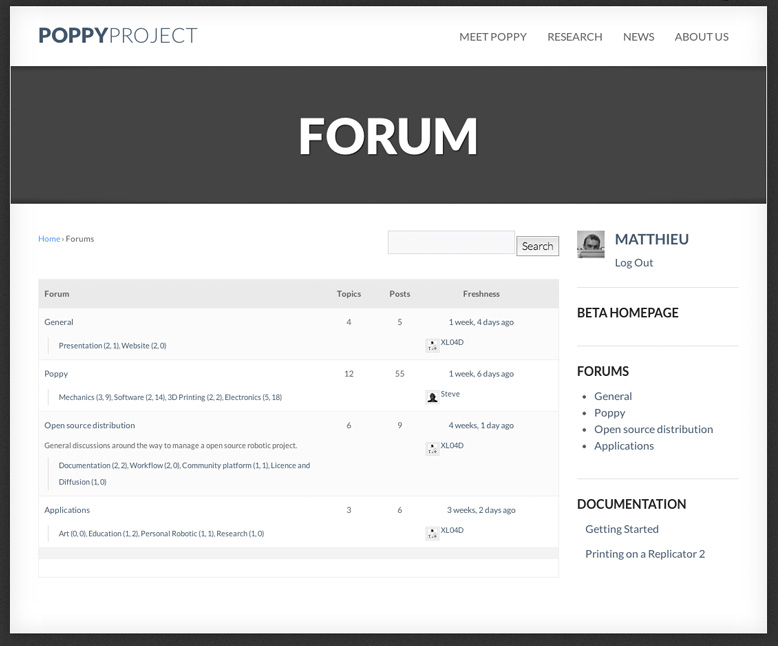
\includegraphics[height=5.2cm]{poppy_forum_bbpress.jpg}}
    \hfil
    \subfloat[][Current Discourse forum]{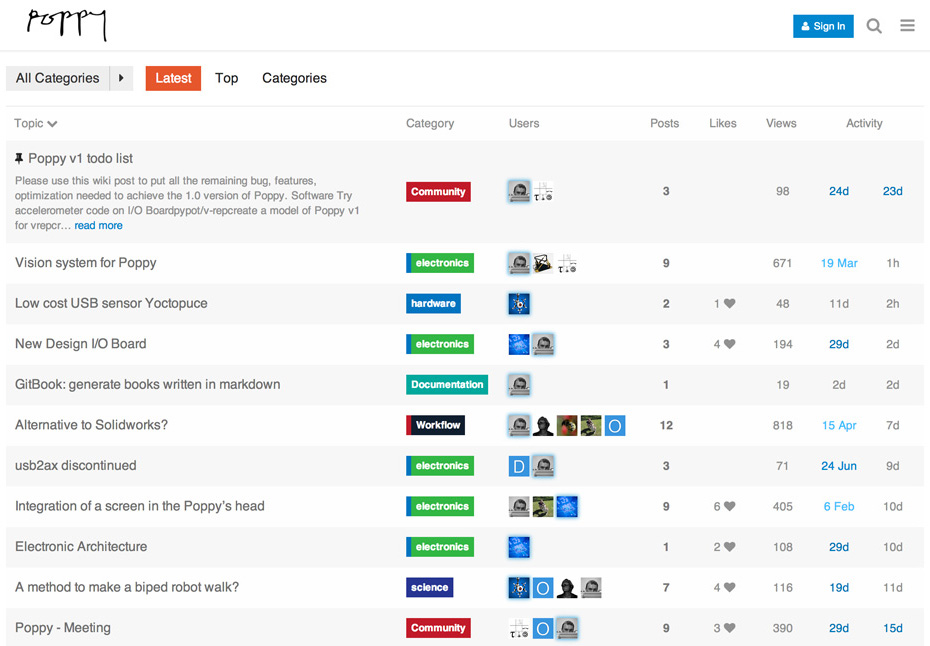
\includegraphics[height=5.2cm]{poppy_forum_discourse.jpg}}
    \caption{Evolution of the forum for the Poppy project}
    \label{fig:poppy_forum}
\end{figure}

Several months ago, we set up a novel forum technology called Discourse\footnote{\url{www.discourse.com}} and created by Jeff Atwood. This forum, available on \url{forum.poppy-project.org} greatly helps us to manage the community, as it is playful and simple (see \figurename~\ref{fig:poppy_forum}). It is so efficient that we began to use it also for our internal discussions about Poppy's development. These discussions are made public so we can merge time between internal and external communication, extending at the same time the openness of the project.

While this technology solves one of our problems, there are still several others. Firstly, we did not find a wiki technology as simple and playful as Discourse, therefore currently the project clearly lacked documentation (except from pypot whose documentation\footnote{pypot documentation: \url{poppy-project.github.io/pypot/}} is complete).

Secondly, as a science project, we naturally decided to use English as the main language for all communication associated with the project. This means the main website for presenting the project, as well as support on the forum and the current documentation. However, as we can see in the \figurename~\ref{fig:poppy_community}, English native speakers only represent one-third of the Poppy community. While English is usually not a problem for Germanic countries, we have been confronted with a lack of contribution from Latin countries on our forum. It is especially the case with French educational and artistic communities who have never contributed to the forum even after the successful experiments we have done (see chapter~\ref{cha:education} and chapter~\ref{cha:art}).

Following the Arduino example, we now made our forum multilingual\footnote(see this topic \url{https://forum.poppy-project.org/t/multi-language-enabled-on-this-forum/304}) by allowing and creating the associated categories for French, German, Italian, Spanish and Portuguese. We are also currently translating the main website. This work has not yet produced results, but we missed the opportunity during the experiments we did, and we certainly have to wait until new experiments in education and art to see if we can actually draw more contribution from non-English speaking participants.

\begin{figure}[tb]
\centering
    \subfloat{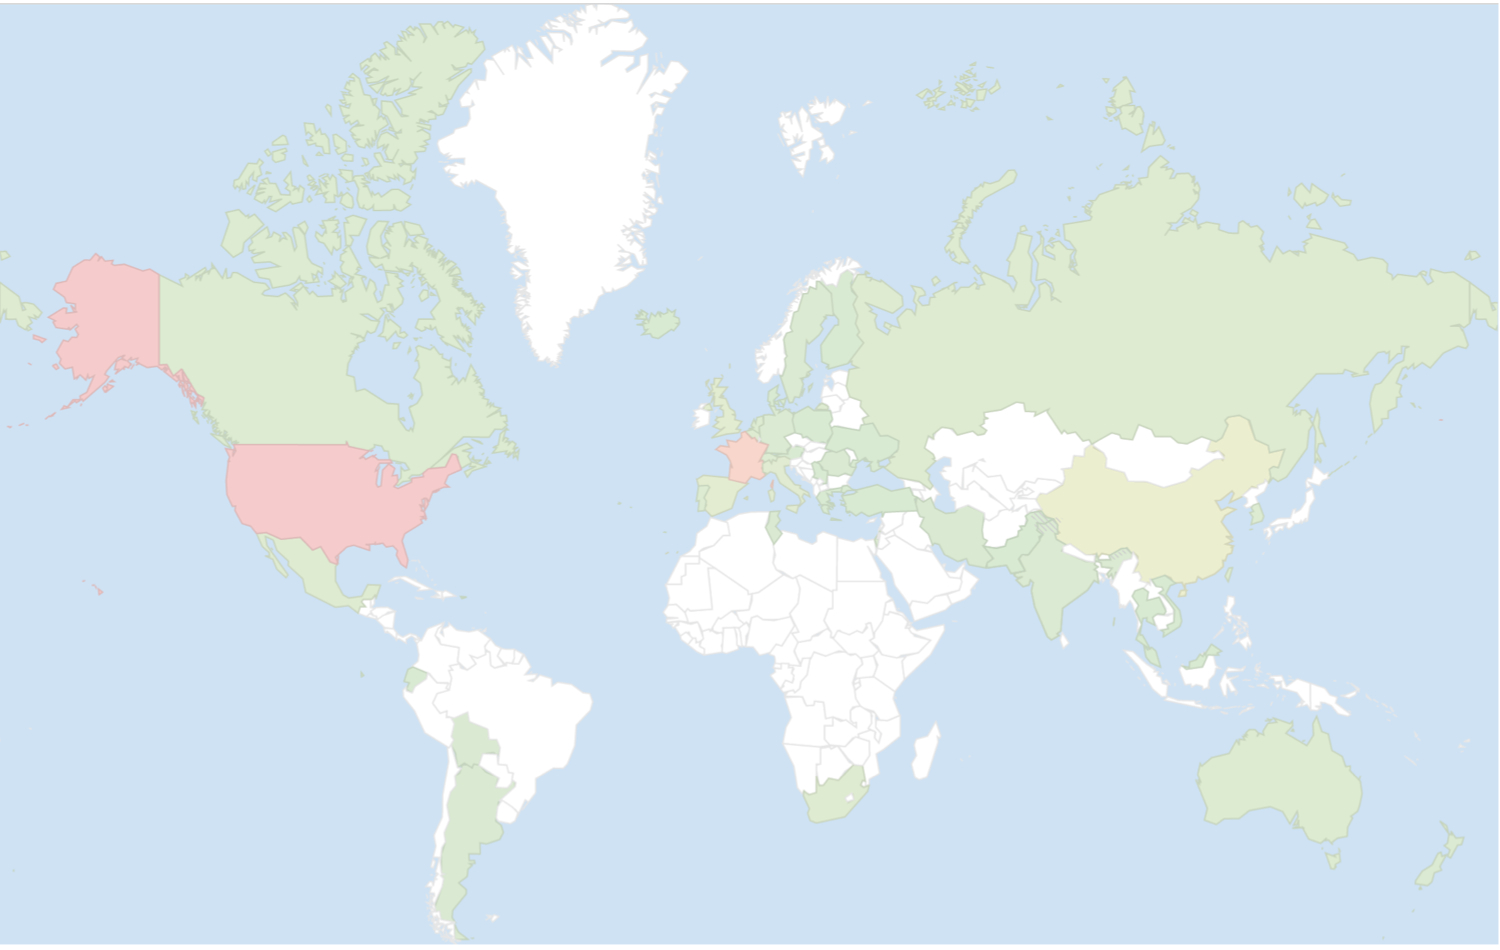
\includegraphics[height=4.5cm]{world_map.jpg}}
    \hfil
    \subfloat{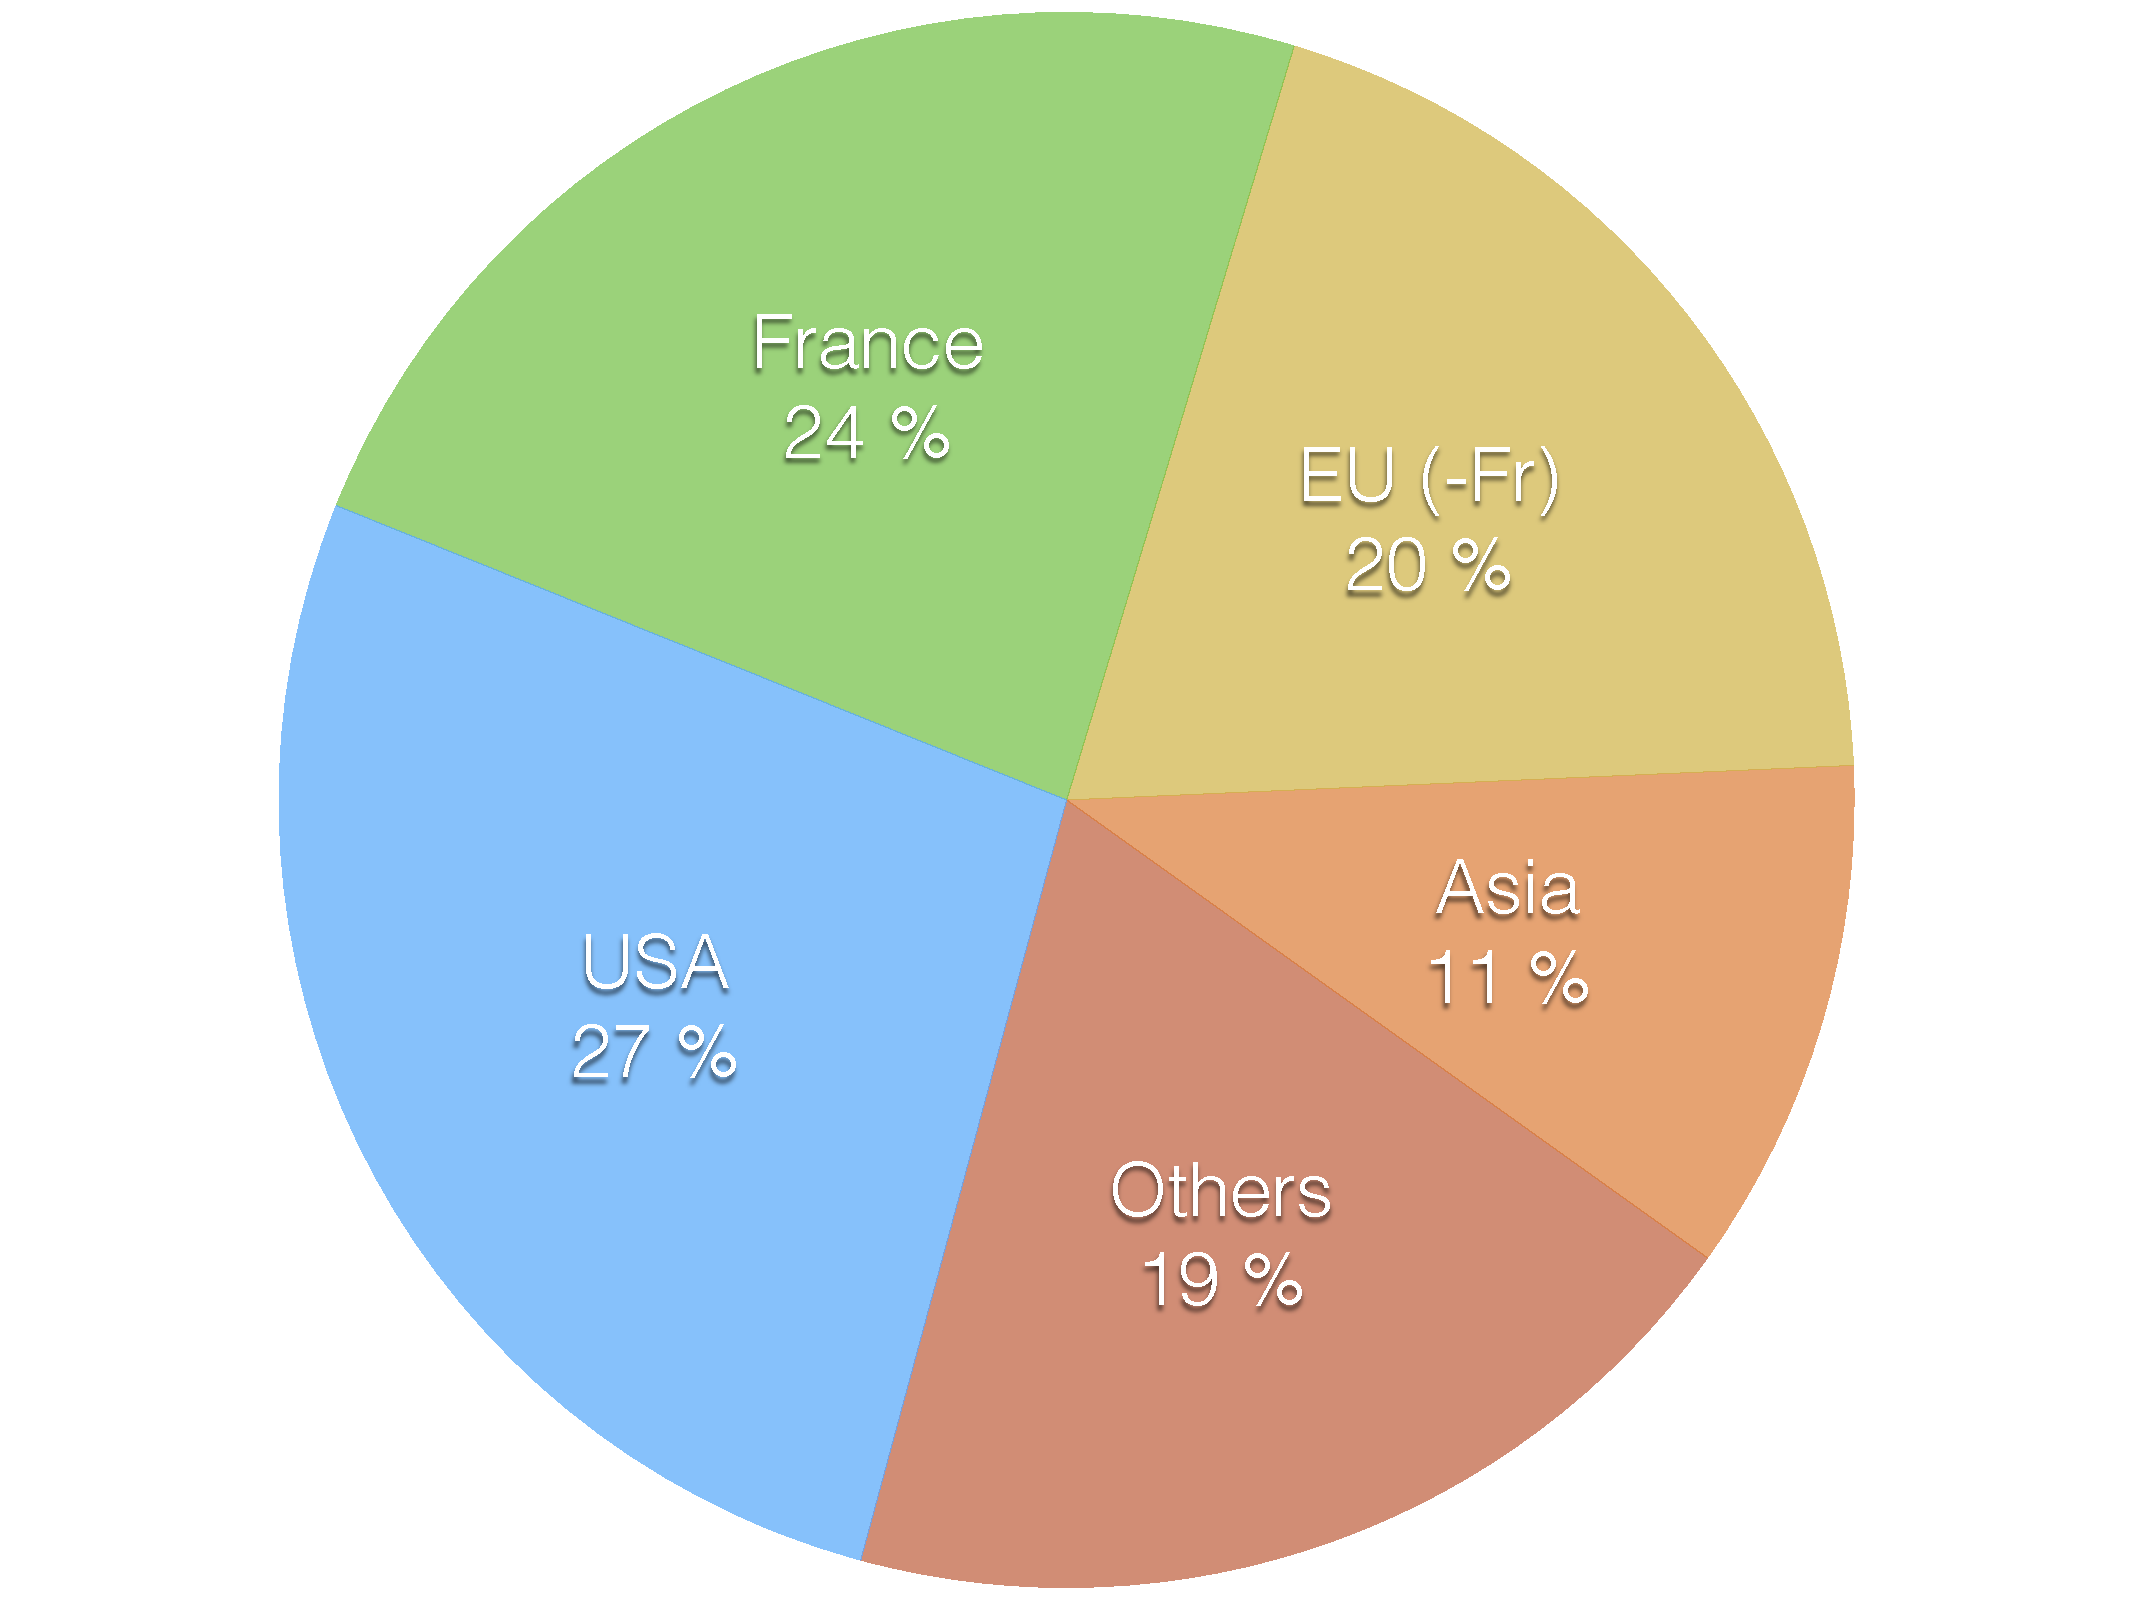
\includegraphics[height=4.5cm]{user_country.pdf}}
    \caption{Activity tracked during October 2013 to February 2014}
    \label{fig:poppy_community}
\end{figure}


Third, creating a multidisciplinary community implies that participants do not speak the same language and do not have the same technical level. Therefore, we will have to improve the accessibility of the project to create a motivational learning curve. This can be achieved thanks to a well-designed interface, playful content and gamification (\cite{deterding2011game} \cite{groh2012gamification}).

Also we have to take into account the fact that people do not read documentation, described as the paradox of the active user in~\parencite{carroll1987paradox}:
\begin{formal}
    Users never read manuals but start using the software immediately. They are motivated to get started and to get their immediate task done: they do not care about the system as such, and do not want to spend time up front on getting established, set up, or going through learning packages.
    The "paradox of the active user" is a paradox because users would save time in the long term by learning more about the system. But that is not how people behave in the real world, so we cannot allow engineers to build products for an idealized rational user when real humans are irrational. We must design for the way users actually behave.
\end{formal}

Jeff Atwood also explained this behaviour in his post on the "just in time theory\footnote{\url{http://blog.codinghorror.com/the-just-in-time-theory/}}" and addressed the problem in Discourse by putting a reminder when a user is going to do something that may be wrong, by summarizing relative topics or forum rules, for example, just when a user is about to post something.

Understanding users’ needs is very complicated, especially as Poppy users can be young students, artists or robotics experts. Therefore a major part of the community is not even aware of basic robotic problems such as motor orientations, the concept of communication buses, the fact motors can burn if too loaded. Thus in addition to complete documentation (for the good students), we will have to work on the “just in time” reminders so other people can easily assemble and use Poppy.
We already explored some solutions for the assembly. For example, motors can be oriented with 16 potential configurations, we need to use one so everyone can share the same robot configuration code (see section~\ref{sec:pypot-robot-abstraction}). We put a directly visible indication on the 3D-printed parts so users can see how the motor has to be oriented (see \figurename~\ref{fig:motor_orientation}).

\begin{figure}[tb]
    \centering
        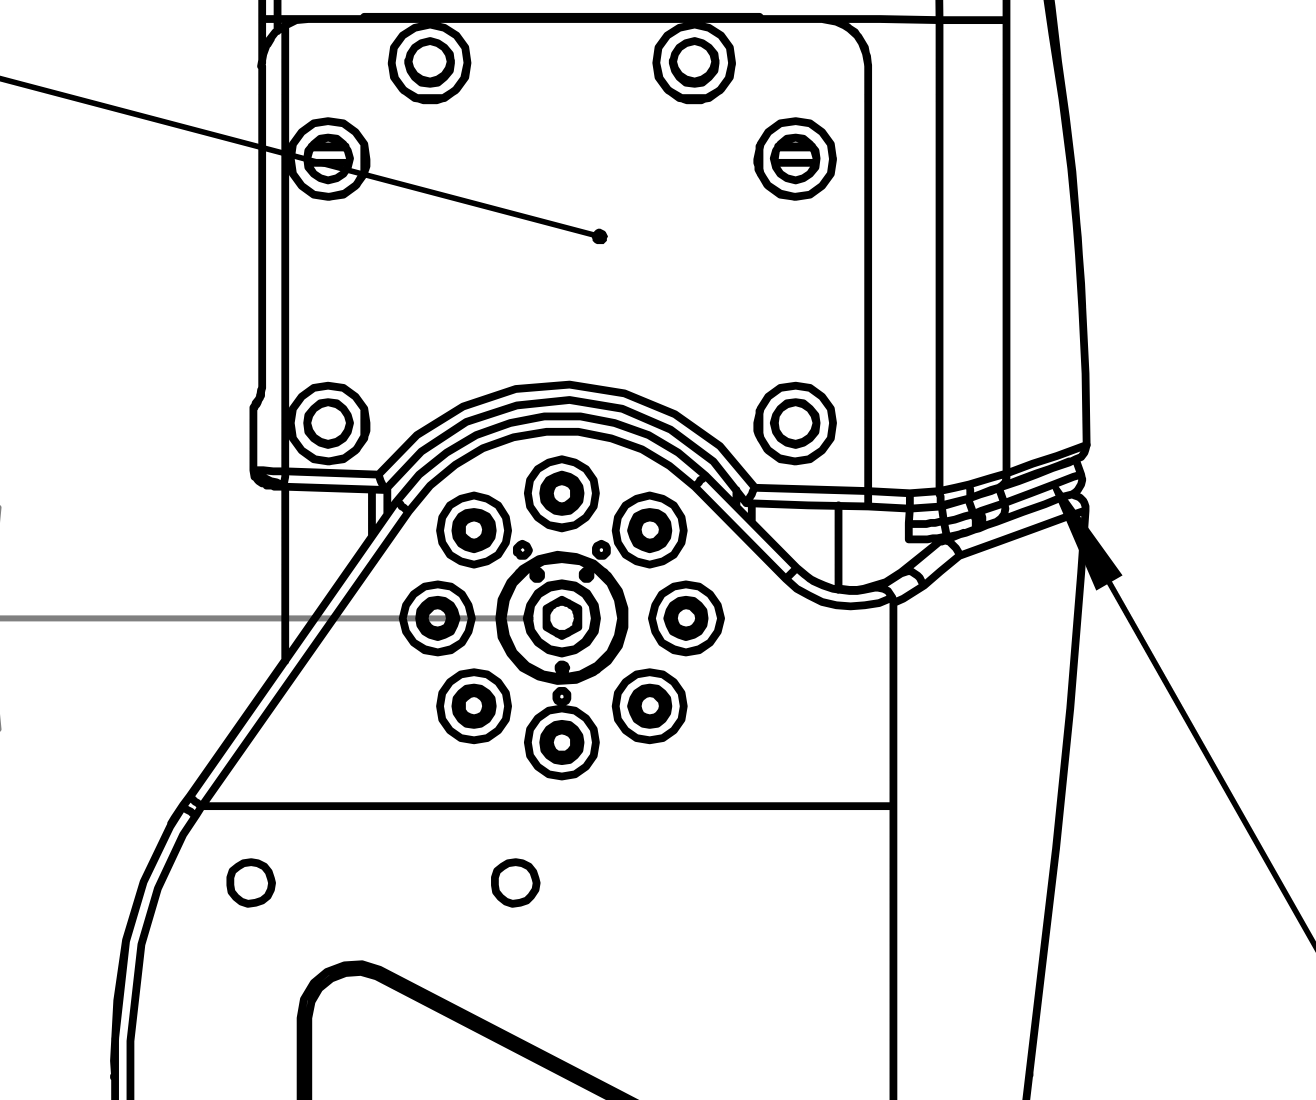
\includegraphics[width=0.6\linewidth]{motor_orientation.png}
    \caption{Image will be updated to be more explicit. Yet we can see the 3 points on the motor axis are also present on the part, it is only required to align these points to be sure that the motor is correctly assembled. It is kind of mechanical “just in time reminder".}
    \label{fig:motor_orientation}
\end{figure}

Yet this work should be propagated on all elements. On electronics devices so users have important information (e.g. max voltage, ground/ VCC orientation) directly printed on the board like Arduino did on their boards. On the software so users can be reminded that the primitive paradigms can create undesired behaviours\footnote{The primitive paradigms: The Good, the Bad, and the Ugly, see section\ref{sec:pypot-primitives-problems}} as well as being informed when the robot is suffering from too much load.

\section{Create relevant educational content} % (fold)

The first experiments we did in education appeared promising (see chapter~\ref{cha:education}). We also received numerous requests from education structures in France as well as around the world. Indeed, robotics is an atypical "science" intrinsically multidisciplinary, merging engineering, computer science, biology, cognition and even humanities. Beyond teaching robotics, it provides a basis for creating an original multidisciplinary course. Also, robots are very motivating tools as they can be incarnated intangible objects.

However this impact cannot rely only on a technological platform, relevant content needs to be created for it to be a real education vector.
For this reason, we are setting up a partnership with ENSAM\footnote{Arts et Métiers ParisTech is a French engineering and research graduate school in the fields of mechanics and industrialization.} and Aérocampus\footnote{REF} to create and evaluate educational content associated with the use of Poppy on the students from baccalaureate -3 to +3 i.e. high-school and bachelor level. All content will be produced and disseminated under Creative Commons and will be composed of ready-to-use sheets of practical experiments with robots, specifying objectives and concrete progress in the classroom; their organization into a coherent and integrated curriculum; and tutorials in the form of videos or multimedia web pages. They may take the form of an MOOC that can be disseminated on the national platform FUN\footnote{REF}. Also being open source, anyone can contribute to its improvement. One particular extension of this work could be an evaluation for self-training through experiments in Fablab.


\section{Improving hardware modularity} % (fold)
\label{sec:improve-hardware-modularity}

As we discussed in detail in this thesis, Poppy has a modular morphology. This modularity is expressed with all the technologies involved. For the mechanics, we use 3D printing techniques allowing producing quick and low-cost parts. For the electronics, we designed a board based on Arduino allowing to easily plug new sensors in. Finally for the software, we built a library using a modular architecture both for the low-level thanks to I/O controllers and for the high-level with primitive paradigms.

As we saw in the chapter~\ref{cha:changing_morphology}, this modularity allows for quick experimentation with morphological variants. This functional modularity seems to be enough to allow a wide range of scientific experiments with Poppy and hopefully have a real scientific impact. However, to have an actual impact in the open source community, technological modularity is essential.

In software, modularity refers to the manner in which a design is decomposed into different "modules". It is based on the notion of interdependence within modules and independence between modules~\parencite{baldwin2000design}. This concept involves two related ideas: the need to allow work on a given module to be carried out without affecting other modules in the design, a concept known as "loose-coupling", and the need for well-designed "interfaces" between these modules~\parencite{maccormack2006exploring}.

The concept of modularity appears as a fundamental property in open source software collaboration. Indeed, code modularity allows the overall project to be divided into much smaller and well-defined tasks that individuals can tackle independently from other tasks and without affecting other aspects of the program~\parencite{narduzzo2008modularity}.

Thus Linus Torvalds, emphasized modularity as a design criterion early in the development of Linux~\parencite{dibona1999open}. Indeed without modularity, it would be improbable that contributors could understand the whole design architecture enough to make a relevant contribution. It would be difficult to add new features or fix bugs without affecting other parts of the design. Linux needed to be modular to attract and facilitate a developer community. Code modularity allows partitioning of work among a global pool of developers and facilitates the recruitment of new contributors, as it reduces their learning curve to a subset of modules rather than the entire project~\parencite{fitzgerald2004critical}.

Various efforts by corporations selling proprietary software products to develop additional products through an open source approach have been undertaken. One of the most visible of these efforts was Netscape's 1998 decision to make 'Mozilla', a portion of its browser source code, freely available. This effort encountered severe difficulties in its first year, only receiving approximately two dozen postings by outside developers. Much of the problems appeared to stem from the insufficiently modular nature of the software: reflecting its origins as a proprietary commercial product, the different portions of the program were highly interdependent and interwoven.

Over twenty years, open source software development has managed to find an efficient workflow. There are now tools, rules and guidelines allowing people to develop new software fluently together.

In hardware, modularity is not as developed as in software because it is not possible to abstract the interface. Hardware components have an overall shape, connector type and position, and so on, which makes it difficult to design an efficient interface.

\begin{figure}[tb]
\centering
    \subfloat[][Arduino form factor]{\includegraphics[height=3.5cm]{arduino-shield.png}}
    \hfil
     \subfloat[][Google Ara project]{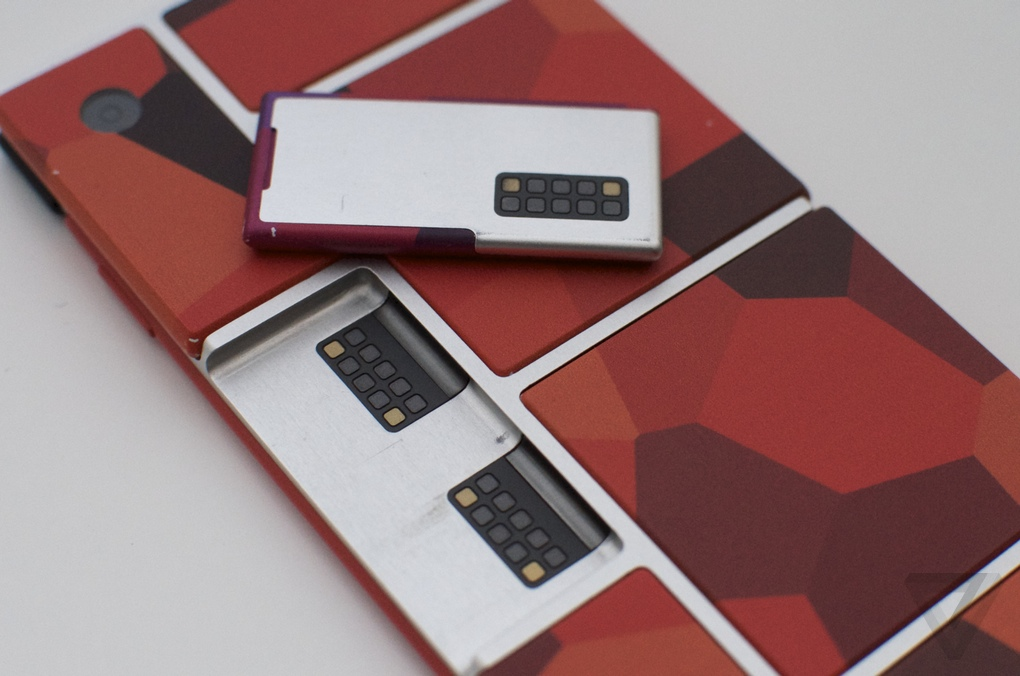
\includegraphics[height=3.5cm]{project-ara.jpg}}\\
    \caption{Examples of hardware modularity achieved so far.}
    \label{fig:hardware-modularity}
\end{figure}

Some projects have already addressed these challenges. For example, the Arduino boards (Uno, Leonardo, Yun, Mega, Due) share the same footprint (i.e. where the main I/O pins are placed), in this way any shield developed for one of these Arduino boards can also be used on other one. This modularity is a lever arm for the community as potential contributors know that the shield they develop and possibly sell will be compatible with several boards and future ones.
Another example is the Google ARA project, it is a smartphone with modular elements. It is possible to change only the processor or the camera without having to change the whole phone. To achieve such a design, they created an interface block (see REF). Therefore, any modules following the interface rules can be plugged on the phone.

% Add the fact that people should be able to easily change a part of the robot

To improve the potential impact of Poppy for the technology we need to follow such ideas. Indeed, the methodology used to build Poppy allows for modularity but the actual hardware design is interdependent. The functioning of each mechanical part depends also on elements connected to it, for example, the way the pelvis is designed changes the mobility of the legs. Also the particular shape of the IO board and the way connectors are placed, are designed to fit in the current design of Poppy's head. It does not prevent the reuse of such components in other projects, but it reduces their relevance.

Thus it would be very useful for a robot platform such as Poppy, made to explore/hack/develop robotics, to easily switch between different technological solutions. On one hand, we could test in minutes completely different morphologies (a new pair of legs for example). On the other hand, and it is maybe the most important point, it would permit the community to develop their own version of any of Poppy's mechatronics systems without having to reconsider the whole robot structure. By Poppy's systems, we mean legs, feet, arms, hands, torso or head.


Our future technological development will be more oriented toward hardware modularity. This work is already under process for the two main aspects of the robot.

\begin{figure}[tb]
\centering
    \subfloat[][IO Module schematics (under production)]{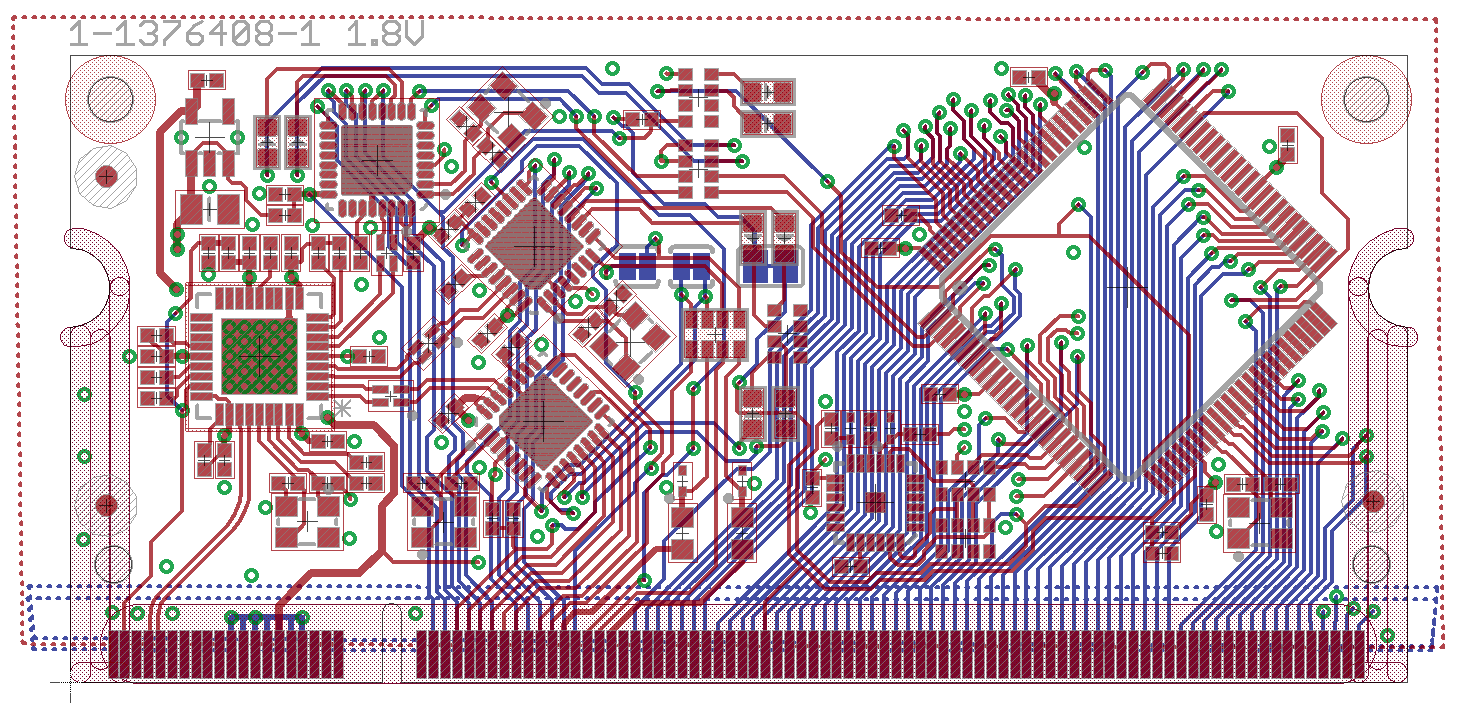
\includegraphics[height=3.5cm]{io-module.png}}
    \hfil
     \subfloat[][Size comparison between the IO board and SO-DIMM format]{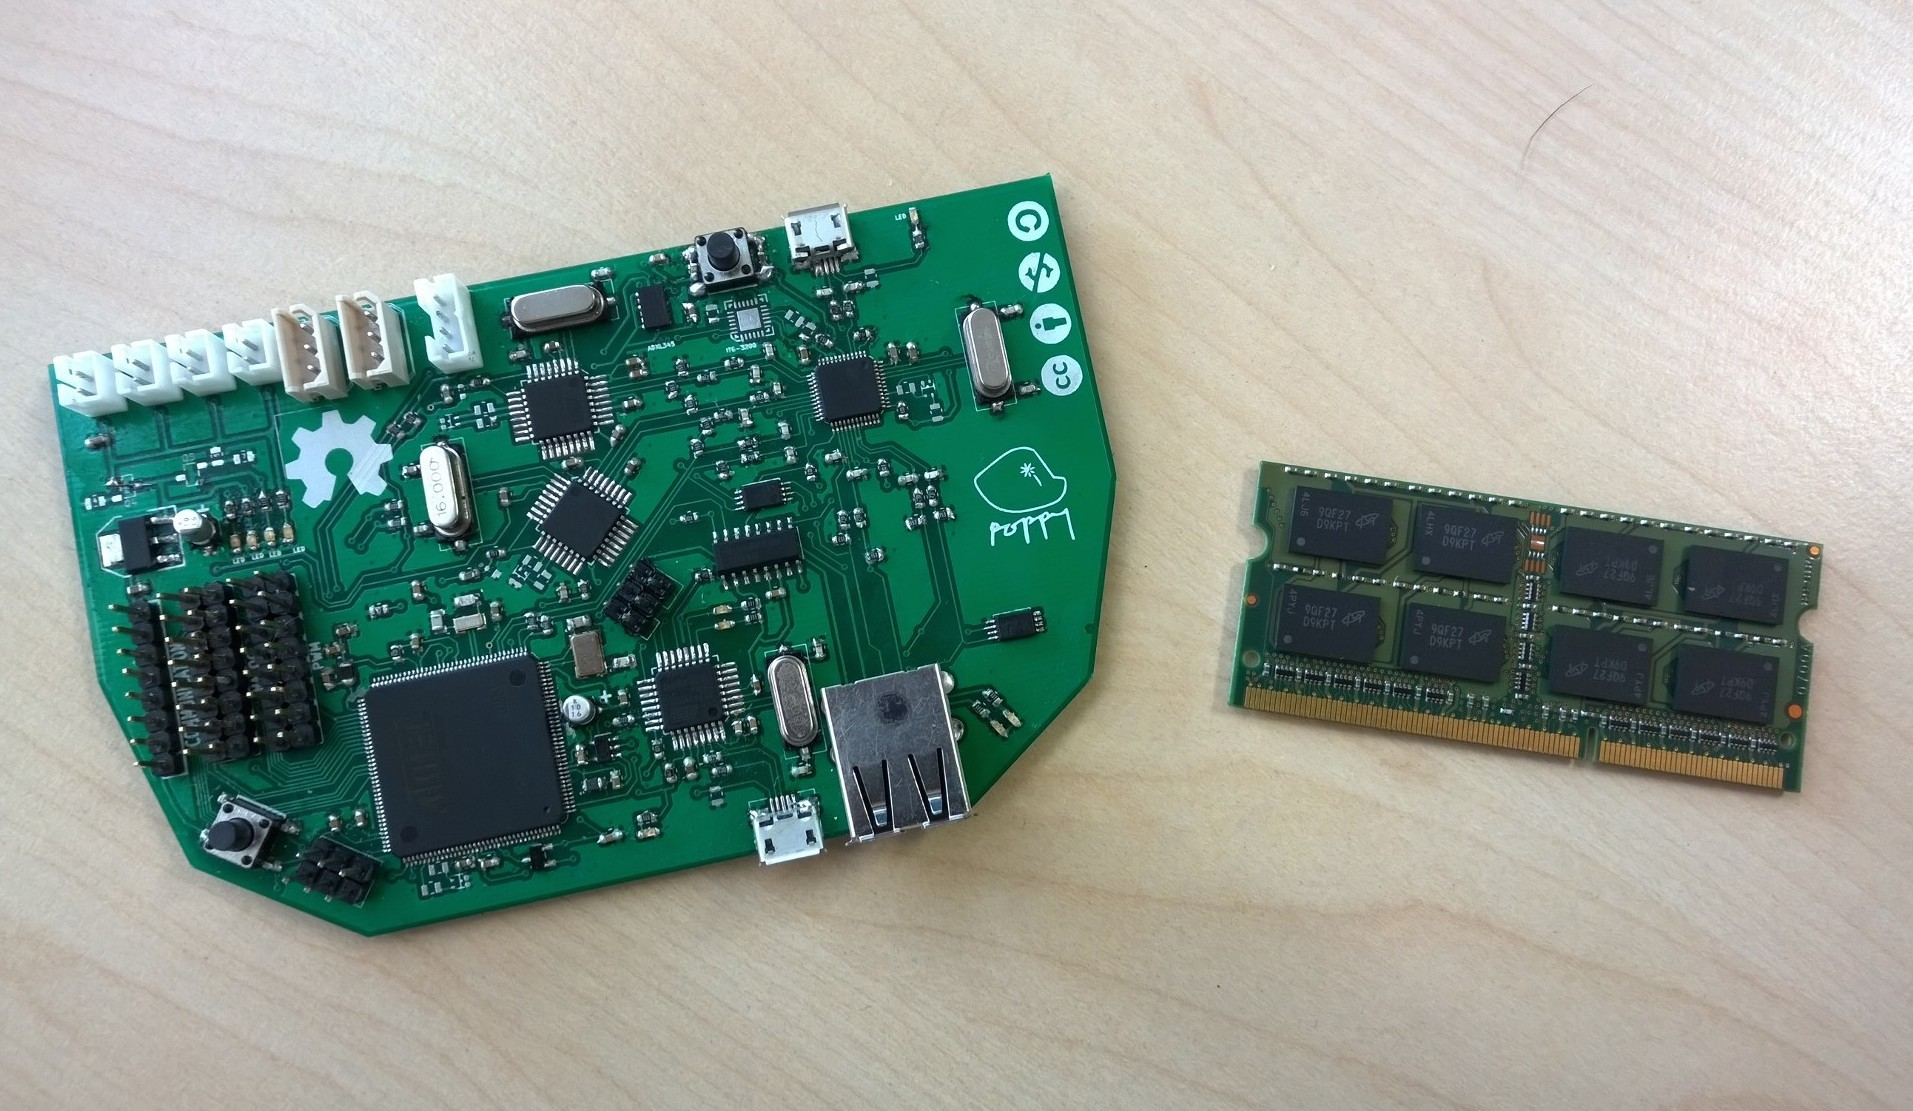
\includegraphics[height=3.5cm]{compare-io-boards.jpg}}\\
    \caption{A novel IO module is under development. This IO module only includes the core components for controlling robots such as Poppy. Its tiny size and standard interface make it easy to embed.}
    \label{fig:poppy-electronic-modularity}
\end{figure}

We are also exploring splitting the electronics into modules. We are working on a new design of the IO board, which will involve 2 boards, one IO module with the core of the technology we need (Arduino, motor control) and a shield with connectors.
While the shield is customized to one robot, depending on the needs and motors used, the IO module is very small and versatile so it can be integrated both in small and big robots.
The design of this IO module has already been done (see \figurename~\ref{fig:poppy-electronic-modularity}) and is based on a DDR2 SO-DIMM format (67x30 mm) with up to 200 pins. This board involves an Arduino Mega with all its GPIO, two modified motor buses compatible for TTL and RS485 communication and an inertial unit MPU6000.


For the mechanics, a first step toward more modularity could be to split the robot into interchangeable sub-modules with defined interfaces. In this way, contributors could create new designs while only having to ensure that the interface is compatible. Therefore anyone could create a whole new head or legs system and distribute it so people could test it on their Poppy.
We would like to suggest these sub-modules: Head (neck + head), Torso (abs, spine, chest), Arms (both from shoulder to hands) and Legs (both, include pelvis, legs, and feet).

Thus, it enables a large range of reconfigurations on Poppy and people are not limited to an evolution of the current design but can create completely new morphology while being compatible with Poppy's other modules.
For example, we could have several locomotive systems such as two legs, one jumping leg, wheels, 4 legs (centaur) or just a static base.

While the overview of the module system seems clear for us, the details are still rather muddled. Typical examples are the arms, where the functional distinction is not clear. In the current version of Poppy, the motor for one of the arms is in the torso. From a functional point of view, it should be integrated into the "arms" sub-modules, but on a practical level it means you cut out a huge part of the torso and will greatly complicate the interface design.

Another point is the pelvis/torso interface, on one hand, it would be simpler to consider the abs motor as the interface, on the other hand, we do not want to enforce having an abs motor for other submodules.

These kinds of submodules still raise a limitation because the interface has a fixed size, which will constrain the overall size of the robot elements. It should be possible to create a bigger robot, maybe up to 120cm high but it will be difficult to have a robot smaller than 60cm while keeping the same interface.


\section{Production/Distribution: an alternative approach} % (fold)

Poppy includes three main parts: its mechatronic structure (skeleton and motors); its electronics; its software.

Reproducing and rebuilding the mechatronic structure is easy: the open-source skeleton can be printed on personal 3D printers (or using online services for higher quality printing), and motors are bought off-the-shelf (motors are currently not open-source, but very standard). Obtaining and using the software is very easy: just download on the Poppy website.

But manufacturing electronics is a bit more challenging. It is not yet possible to produce electronics components at home, and many institutional users do not have the skills or motivation to do so. There are some kick-starter projects on the way to facilitating the process, yet they are not ready and will not be ready for a couple of years. The current classical approach to building and distributing these electronics boards is to raise funding allowing for hundreds of boards to be manufactured, which can then be sold by a distribution company. Thanks to new online platforms such as CircuitHub it is easy to produce anything from a single model to thousands of boards. Yet the cost is exponentially decreasing and unlike 3D printing. But a French research institute like Inria is not a distributor, it cannot raise funding to "mass" produce electronic components before reselling them. It is not even legally allowed to do so.

Indeed, the mission of a research team at Inria is to do research, and find ways to apply and transfer the results of this research, but not directly to produce and sell a commercial product. If a commercial products emerge from our research, one way to take advantage of it is to create a start-up company which will set up a business plan around it, probably based on production in Asia and then worldwide distribution to research laboratories, universities and fab labs (see \figurename~\ref{fig:classic})

\begin{figure}[tb]
    \begin{center}
        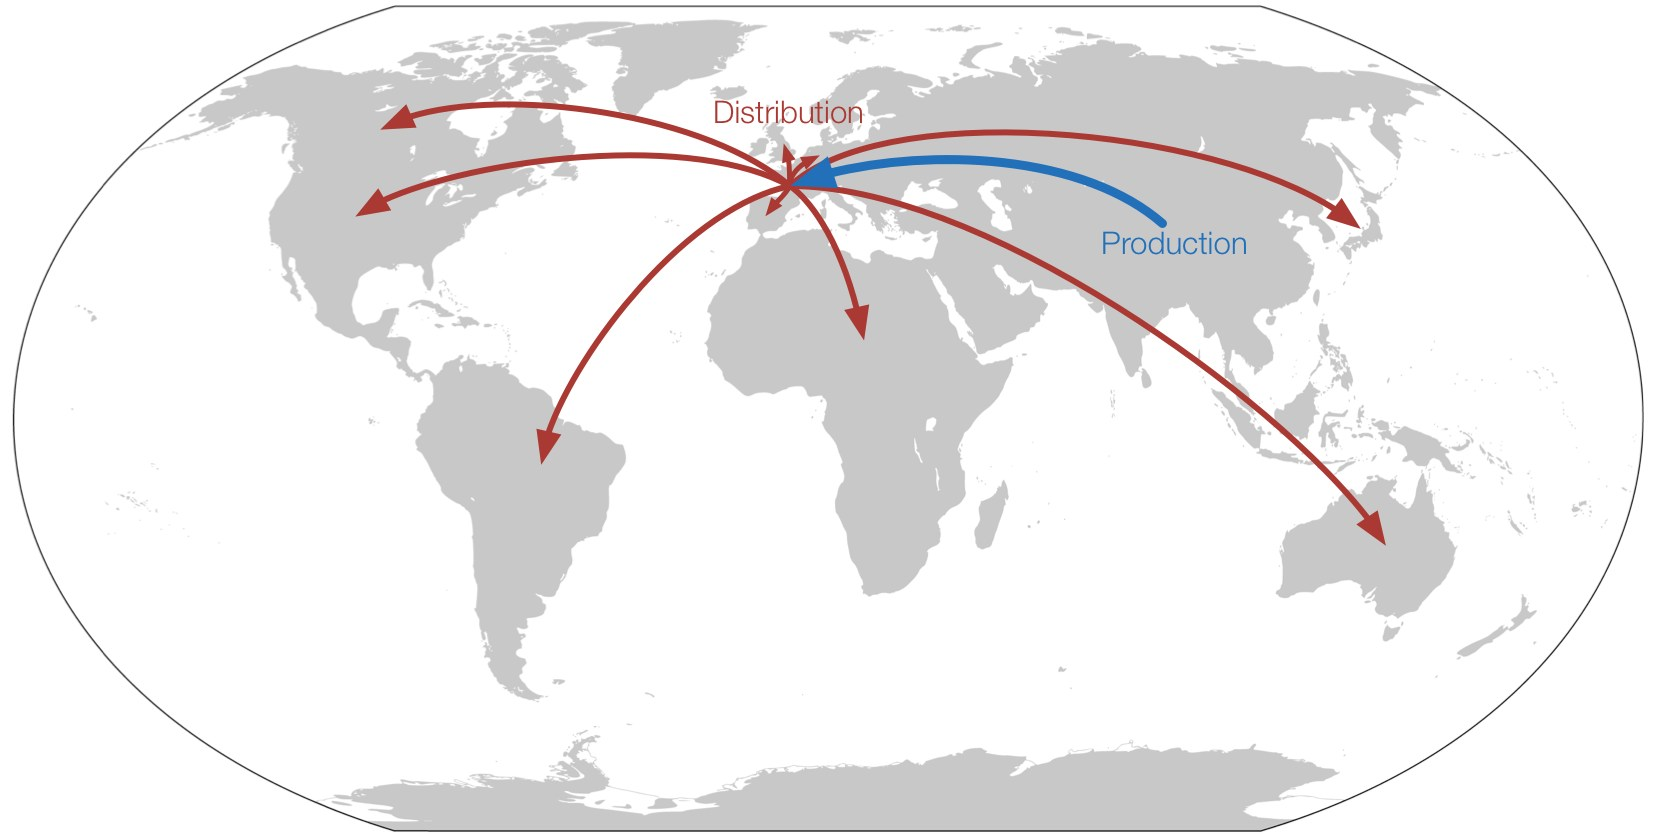
\includegraphics[width=\linewidth]{classic_production_distribution.jpg}
    \end{center}
    \caption{Classical approach for technological production and distribution}
    \label{fig:classic}
\end{figure}

But Poppy is not designed to be a standard commercial product. While it might foster the creation of an economic ecosystem and jobs, its main purpose is to become an educational tool that remains open, as well as rather a low cost and easily reproducible. If the goal had been to make it profitable, it would be necessary to sell it at a much higher price. The robot would not be as accessible at it needs to be to ensure the achievement of its scientific diffusion and educational missions... We would lose the intrinsic purpose of Poppy.

That being said, some users (e.g. artists) might want to obtain and use an already fully assembled Poppy robot and the sale of already prepared kits can be a lever arm for the diffusion of the platform in the research community.
Also, one of the main purposes of Poppy is to be hacked and modified.  While some people have all the tooling needed, others may find useful to have external support, even if they are charged for the service.

On one hand, the use of classic distributors is, of course, the most direct solution and such a process is already underway to permit the commercialization of Poppy kits by the end of this year. On the other hand, there are novel emerging actors who could add more sense to the distribution of Poppy.


\subsection{Toward local open factories} % (fold)

Meanwhile, the "makers revolution" is gaining momentum~\parencite{anderson2012makers} and more and more Fablabs are created around the world. As one of the main missions of Poppy is to be a novel educational platform, Poppy could become a popular platform used, hacked, and transformed within the natural FabLab activities. But also, and this is the direction explored below,  it would make sense that Poppy, as a whole or subsets of its components, be produced and distributed by Fablabs, and thus becoming a tool used by Fab Lab to develop and solidify the economic ecosystem in which they live.

An original and constructive organizational process would be to take advantage of the production phase for educational purposes. In this context, each fablab would have the possibility to produce, assemble and sell Poppy to local actors (see Figure \ref{fig:world_fab}), while the production phase could become a training resource for using 3D printing techniques and manufacturing electronic circuits, and  later on the constructed platforms would be sold.

\begin{figure}[tb]
    \begin{center}
        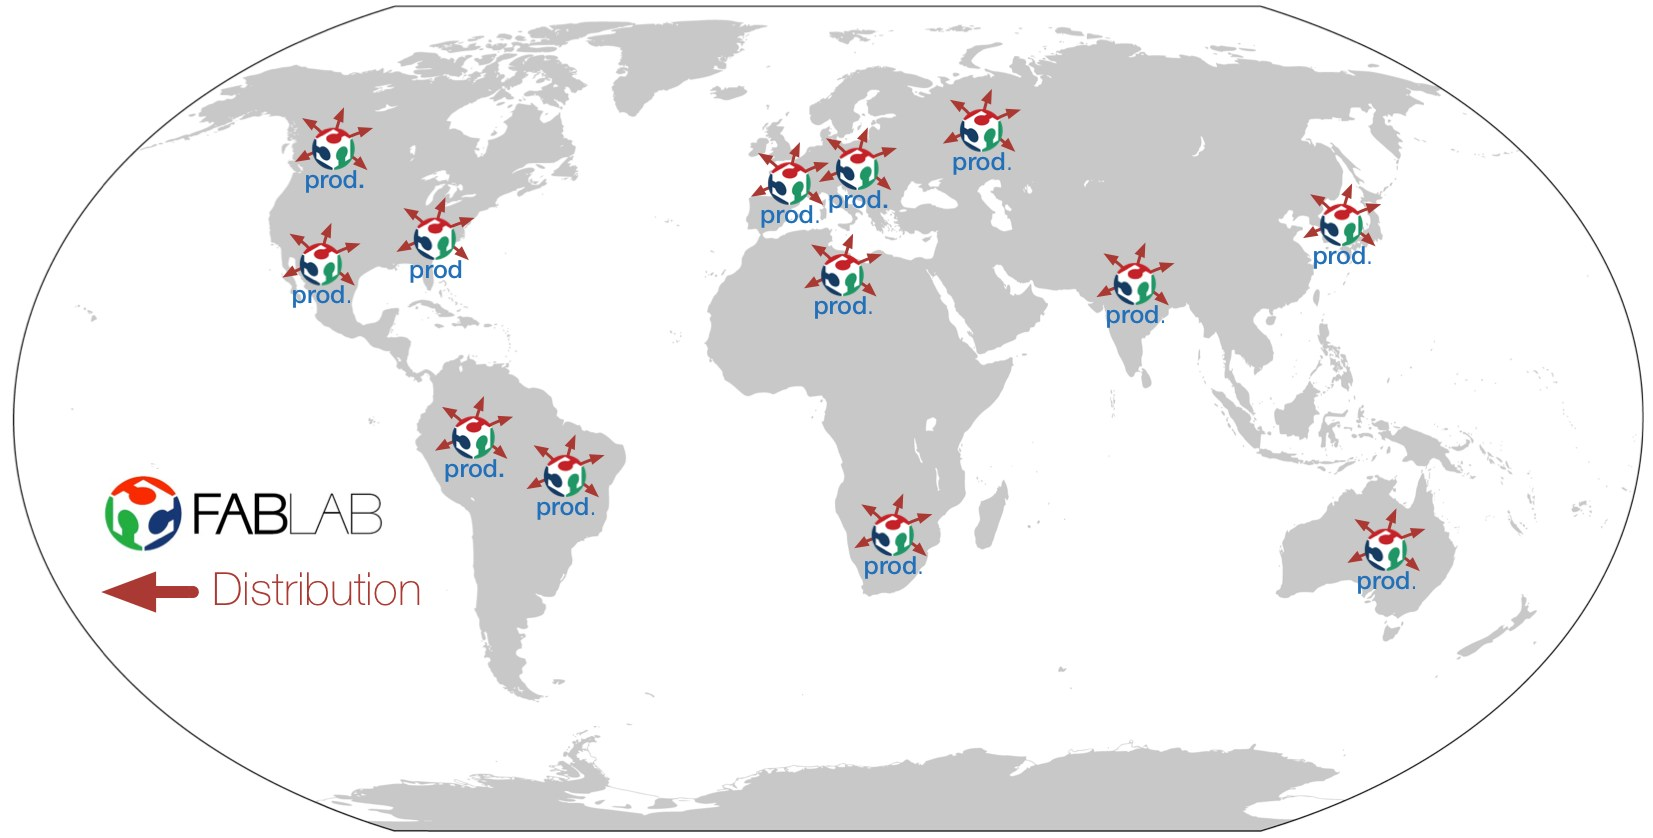
\includegraphics[width=\linewidth]{fabusine_distribution_world.jpg}
    \end{center}
    \caption{Local production and distribution by Fablabs}
    \label{fig:world_fab}
\end{figure}


Also in a context where fab labs need to find an economic model, several sources of income may be found thanks to the distribution of platforms such as Poppy. The first and most obvious one is the sale to local actors of fully-assembled and functional Poppy robots produced by the Fablab. But a more advanced model could emerge. Poppy is a development robotic platform: it means that it can and will be broken, meaning that Fablabs may extend their commercial offers. Among them we can cite:

\begin{itemize}
    \item Ensure technical support (repairs, upgrades, ...) and maybe sell maintenance contracts to labs/school/university and even other third party FabLabs.
    \item Provide a customization service to adapt Poppy to specific needs (e.g. a university or high school that would like to have a Poppy on wheels rather than legs)
    \item For an event or artist residency: the FabLab could rent a robot and provide a technician,
    \item Propose professional training for 3D printing to companies
\end{itemize}

From these kinds of interactions, links and collaboration between local actors and Fablabs may emerge, leading to other potentially funded projects.

\subsection{Promote local collaboration} % (fold)

Beyond the act of production and sales, Poppy could become a pretext for promoting the linkage and exchange between local actors from multiple backgrounds. At the scale of a city or region, we can easily imagine a distribution of roles where several FabLabs could collaborate to build and distribute different parts of Poppy depending on their motivations, skills and equipment.
Also, it helps to connect the fablabs with local actors, public/private research labs, companies, schools/universities or artists (see Figure \ref{fig:local_synergy})

\begin{figure}[tb]
    \begin{center}
        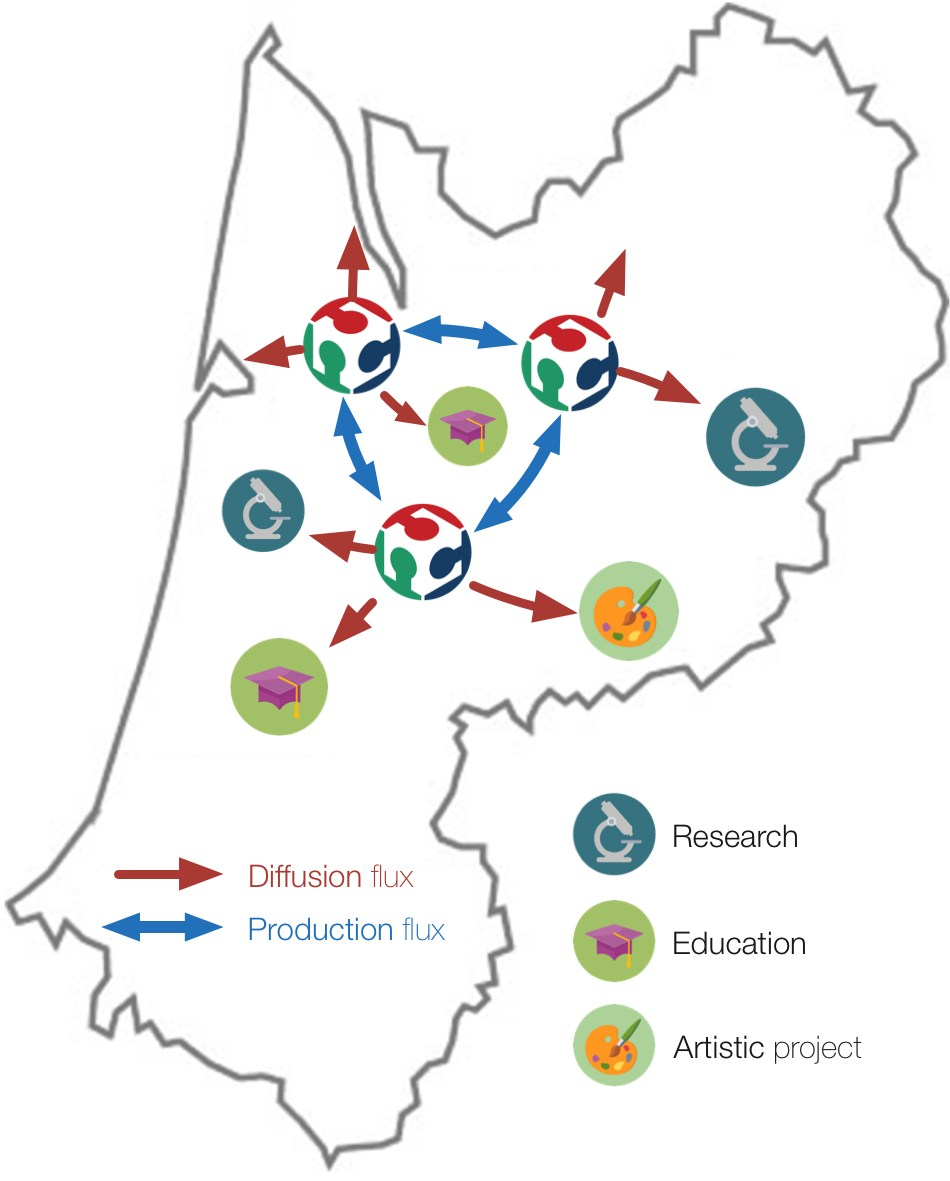
\includegraphics[height=10cm]{fabusine_local.jpg}
    \end{center}
    \caption{A synergy can emerge between Fablabs and local actors}
    \label{fig:local_synergy}
\end{figure}

\subsection{What is the role of the Flowers research team in such a process? } % (fold)

The Flowers research team's role remains essential. As the founders, designers and leaders of both the technological platform and its surrounding philosophy of openness and innovation, the Flowers team continues to improve the platform, take a central role in animating the community of users, and design new uses with scientists, educators, “geeks” and artists. Within this process, the Flowers team also coordinates the growth of the community of contributors and users and designs strategies to ensure both the quality and sustainable development of the platform and its use.

Among the tools used by the Flowers team to ensure such quality and sustainable development is the control of the "Poppy" brand, and through policies/charters:

\begin{itemize}
\item The "Poppy" brand is owned by Inria, and the use of the brand by third parties like FabLabs will only be possible through agreements ensuring that the Poppy project’s policies and philosophy are implemented;
\item Agreements take the form of charters/policies between Inria and FabLabs specifying guidelines to follow to ensure quality and protect the interests of each party (Inria, FabLab, users).
\end{itemize}

On the Inria side, the creation of a spin-off association whose role would be to  oversee the technological development, community management, and quality control, is under consideration.



Therefore, Poppy can be one of the first projects launching this new kind of production and distribution process. Over recent months, we met several of the main French FabLabs. While they are quite enthusiastic about this idea, the organization is not completely ready to go in this way and we will certainly have to use both ways by relying also on classical robots distributors.





\section{Open source force control actuator} % (fold)
\label{sec:open_sourcing_the_robotic_actuations}

All the development we have done for Poppy has been released under open source licenses; the mechanical structure and electronics boards are under creative commons licenses and the pypot control library is distributed under GPL license. These various technological bricks allow for new experiments on the role of morphology to be explored, and foster a creative environment for students and artists. Yet a very important technology brick remains closed: robot actuation.

The Robotis Actuators are expensive (more than 60\% of the cost of the robot), proprietary and no modification is permitted either to the low-level control or the hardware. Furthermore, these actuators are limited as they use a classical position control based on PID and do not permit force control.

The technical limits are firstly problematic for scientific reasons. Indeed, the actuator properties are elements that it must be possible to experimentally control. This is not possible with the Robotis ones, beyond tuning the PID controller values and estimating the maximum output torque. In addition, these actuators act as a black box, we do not have any way of guaranteeing or controlling how the tuning of some parameters actually changes the actuator behaviour. For example, parameters such as the delay and the internal loop frequency are very important when we explore reinforcement learning. Indeed, the algorithm needs to have a controlled synchronization between action and observation, and we were confronted with this issue while exploring biped learning with Poppy.

Secondly, the latest scientific work in the robotics field seems to show the efficiency of force control actuators over position control in creating robots able to act robustly in the real world (e.g. Boston Dynamics robots, MIT Cheetah). Hydraulic and pneumatic actuators are too complicated to be integrated in small and safe robots, but technology based on series elastic actuators\footnote{The series elastic actuation~\parencite{pratt1995series} is a technology based on adding a spring between the motor output and the actuator output. The offset between the motor position and the actuator output is proportional to the external force applied (Hooke law). It is a simple, yet effective way of obtaining direct force measurements at the actuator output. Then a controller can drive the motors following the force feedback to create the desired output torque.} or impedance controls seem very promising.

% The impedance control is ...

% \begin{figure}[tb]
%     \centering
%         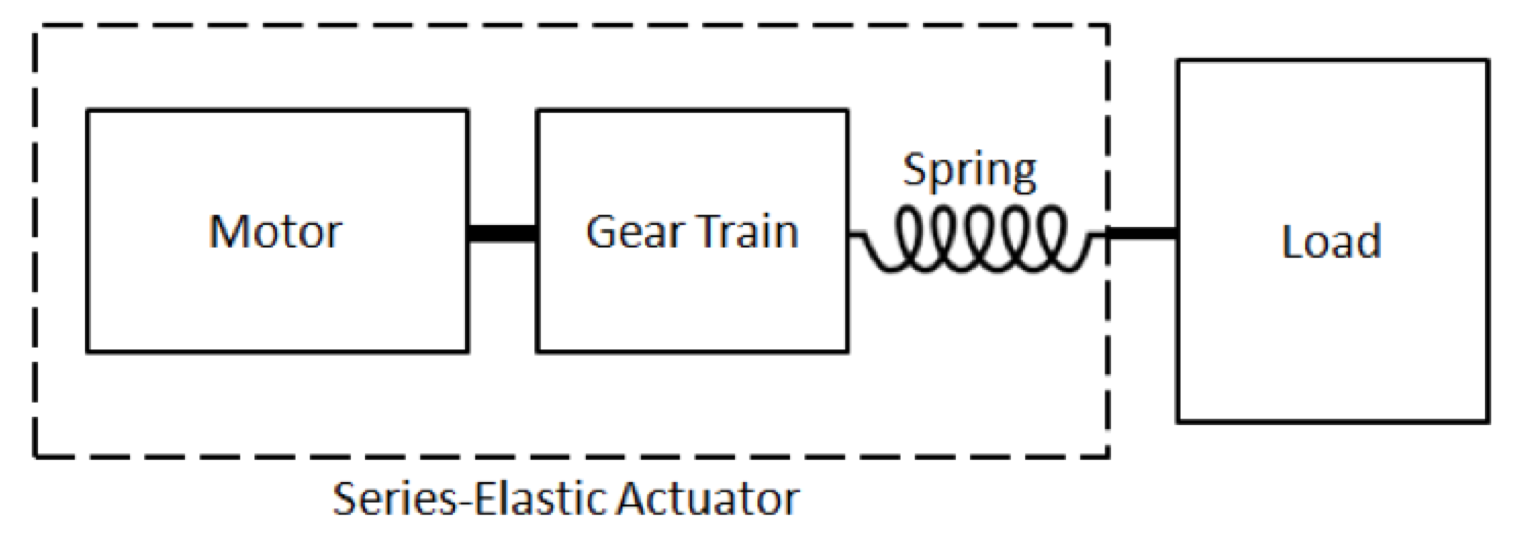
\includegraphics[width=0.8\linewidth]{SEA_basic_principle.png}
%     \caption{}
%     \label{fig:SEA-principle}
% \end{figure}

% These simple technologies have been successfully implemented in several robots ...


Although there are numerous robots based on control impedance or SEA actuators, to our best knowledge, there is no project currently trying to create open source force-controlled actuators. Nevertheless, there are some open source projects to create open source servomotors called open servo and supermodified, yet they only address the electronic parts by offering open source electronic boards compatible with low-cost RC servomotors.


Thus, an important challenge we have already committed to is to create novel open source actuators allowing force control. Inria is supporting this 2-year project and two engineers have been hired for its development. The plan is to first create open source motors equivalent to the Robotis ones, then create a force control module. All the work, mechanics, electronics and software control will be released with open source licenses. In addition, special attention will be focused on creating 3D printable element so users can hack the actuator’s mechanics.

On a scientific level, this actuator will permit free exploration of robot control with an open source control library, allowing to use classical PID control or even to implement a more exotic one.

Finally, we will try to keep as low a cost as possible to increase the potential impact in the robotics field. In particular, using these actuators, we hope to create either a cheaper version of Poppy or a more advanced one, implementing force control for a similar cost.



